\section{Durchführung}
\label{sec:Durchführung}

Es wird der in Abbildung \ref{fig:aufbau} dargestellte Versuchsaufbau verwendet. Zusätzlich
ist dieser durch einen Aufbau aus Bleiblöcken abgeschirmt. Ein weiterer Bleiblock mit Bohrung
dient als Halterung und Fokussierung der $\ce{^{137}Cs}$-Strahlenquelle.\\

Es wird ein Szintillationsdetektor verwendet. In diesem befindet sich ein Szintillationsmaterial, welches
durch die einfallende Gammastrahlung angeregt wird und Licht in Form von Fluoreszens emittiert.
Dieses Fluoreszenslicht hat eine geeignete Wellenlänge, um über den Photoeffekt Elektronen aus 
der Messelektrode zu lösen. \\

Im Photomultiplier lösen sie Elektronenkaskaden aus, welche proportional zur
Eingangsenergie gemessen werden können. Das Signal muss eine Diskrimminatorschwelle übersteigen, durch welche
der unerwünschte Hintergrund kosmischer- und Umgebungsstrahlung oder des thermischen Dunkelstroms herausgefiltert wird.
Schließlich histogrammiert der Multichannelanalyzer das Signal nach seiner Stärke und ordnet es in Kanäle ein.

\vspace{-5pt}
\begin{figure}[H]
    \centering
    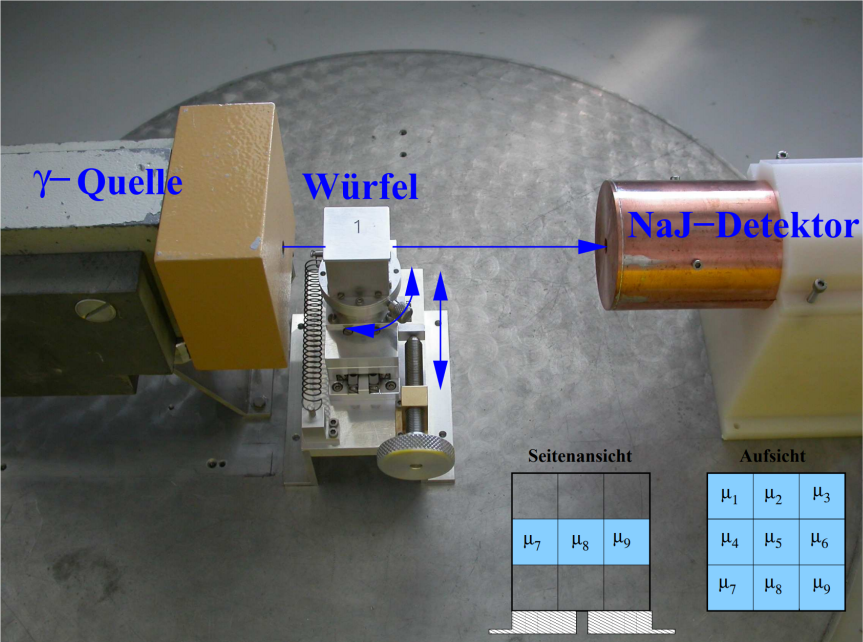
\includegraphics[scale=0.3]{content/aufbau.png}
    \vspace{-10pt}
    \vspace{3pt}
    \caption{Versuchsaufbau der Messung \cite{alt}.}
    \label{fig:aufbau}
\end{figure}
\vspace{-10pt}

Zwischen Strahlenquelle und Detektor kann über eine Justiervorrichtung die Probe in den Strahlengang geschraubt 
und ausgerichtet werden. Es liegen verschiedene 
$\SI{3}{\centi\meter} \times \SI{3}{\centi\meter} \times \SI{3}{\centi\meter}$-Würfelproben vor.
Würfel 1 besteht nur aus dem Aluminiumgehäuse, das für alle Würfelproben außen vorliegt.
Würfel 2 und 3 bestehen aus einem Metall und Würfel 4 und 5 bestehen aus 27 
$\SI{1}{\centi\meter} \times \SI{1}{\centi\meter} \times \SI{1}{\centi\meter}$-Würfeln aus je zwei verschiedenen Metallen.
Die Metallauswahl besteht aus Aluminium, Blei, Eisen, Messing und Delrin.\\

Der Versuch startet mit einer Nullmessung der Intensität $I_0$. Danach werden die abgeschwächten Intensitäten $I_i$
der mittleren Schichten der Würfel 1, 2, 3, und 4 oder 5 aus verschiedenen Winkeln in der in Abbildung \ref{fig:würfel}
dargestellten Schnittgeometrie gemessen.

\vspace{-5pt}
\begin{figure}[H]
    \centering
    \includegraphics[scale=1.2]{content/würfel.pdf}
    \vspace{-5pt}
    \caption{Die verschiedenen Schnittgeometrien der Tomographie.}
    \label{fig:würfel}
\end{figure}
\vspace{-5pt}

\vspace{5pt}
Diese lassen sich zusammenstellen zu der Matrix 
\vspace{5pt}

\begin{equation}
    A =
    \begin{pmatrix}
        0 &         \sqrt{2} &  0 &         \sqrt{2} &  0 &         0 &         0 &         0 &         0           \\ 
        0 &         0 &         \sqrt{2} &  0 &         \sqrt{2} &  0 &         \sqrt{2} &  0 &         0           \\ 
        0 &         0 &         0 &         0 &         0 &         \sqrt{2} &  0 &         \sqrt{2} &  0           \\ 
        1 &         1 &         1 &         0 &         0 &         0 &         0 &         0 &         0           \\
        0 &         0 &         0 &         1 &         1 &         1 &         0 &         0 &         0           \\ 
        0 &         0 &         0 &         0 &         0 &         0 &         1 &         1 &         1           \\ 
        0 &         \sqrt{2} &  0 &         0 &         0 &         \sqrt{2} &  0 &         0 &         0           \\ 
        \sqrt{2} &  0 &         0 &         0 &         \sqrt{2} &  0 &         0 &         0 &         \sqrt{2}    \\ 
        0 &         0 &         0 &         \sqrt{2} &  0 &         0 &         0 &         \sqrt{2} &  0           \\ 
        0 &         0 &         1 &         0 &         0 &         1 &         0 &         0 &         1           \\ 
        0 &         1 &         0 &         0 &         1 &         0 &         0 &         1 &         0           \\ 
        1 &         0 &         0 &         1 &         0 &         0 &         1 &         0 &         0           
    \end{pmatrix}
\end{equation}

\vspace{60pt}
